\documentclass[crop,tikz,convert={outext=.svg,command=\unexpanded{pdf2svg \infile\space\outfile}},multi=false]{standalone}[2012/04/13]
\usepackage{tikz}
\usepackage{pgfplots}

\usetikzlibrary{arrows,shapes,positioning}
\begin{document}
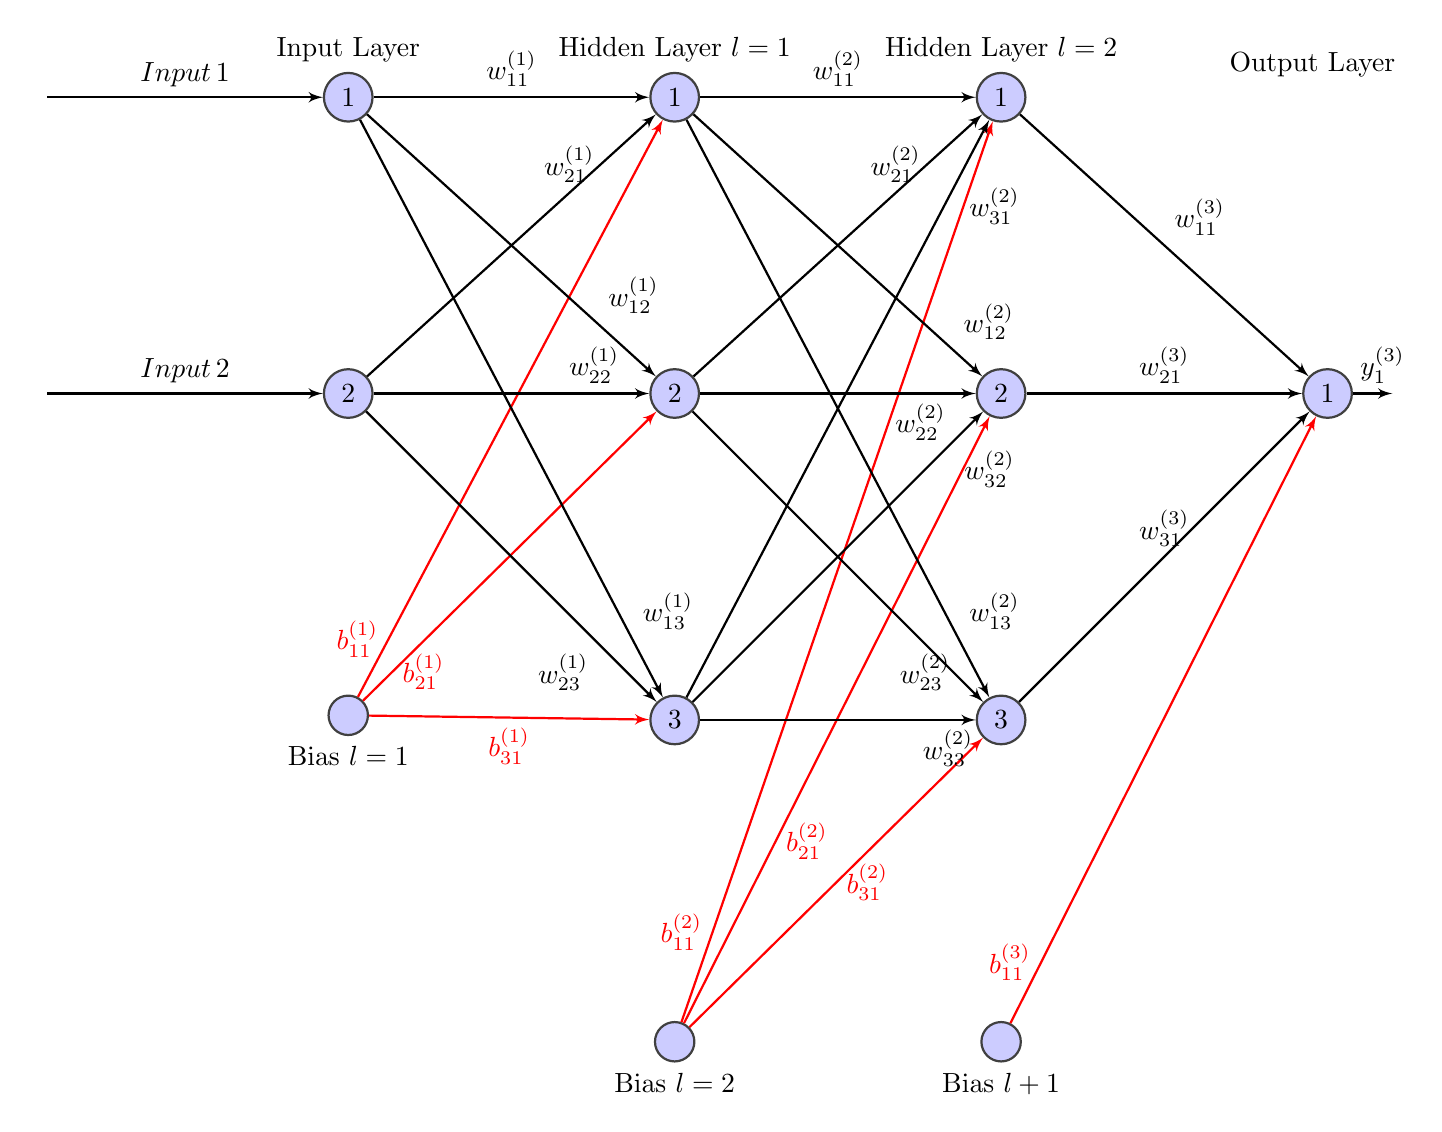
\begin{tikzpicture}[->,>=latex',shorten >=0pt,auto,node distance=3.5cm,
                    thick]
\tikzstyle{komp}=[rectangle,thick,draw=black!75,fill=black!0,minimum size=10mm]
\tikzstyle{sum_punkt}=[circle,thick,draw=black!75,fill=black!0,minimum size=3mm]
\tikzstyle{black_point}=[circle,thick,inner sep=0pt,draw=black!75,fill=black!100,minimum size=1mm]
\tikzstyle{get}=[circle,thick,draw=black!75,fill=black!0,minimum size=5mm]
\tikzstyle{agt}=[rectangle,thick,draw=black!75,fill=blue!25,minimum size=10mm]
\tikzstyle{komp2}=[rectangle,thick,draw=black,minimum size=10mm]
\tikzstyle{mot2}=[circle,thick,draw=black!75,fill=blue!20,minimum size=5mm]

\node[] (black_point_vor_regler) {};
\node[] (black_point_vor_regler1) [below=of black_point_vor_regler] {};

\node[mot2, align=center,label=Input Layer] (input1) [right=of black_point_vor_regler]{1};
\node[mot2, align=center] (input2)[right=of black_point_vor_regler1] {2};
\node[mot2, align=center,label={Hidden Layer $l=1$}] (hidden1)[right=of input1] {1};
\node[mot2, align=center] (hidden2)[right=of input2] {2};
\node[mot2, align=center] (hidden3)[below=of hidden2] {3};

\node[mot2, align=center,label={Hidden Layer $l=2$}] (hidden11)[right=of hidden1] {1};
\node[mot2, align=center] (hidden12)[right=of hidden2] {2};
\node[mot2, align=center] (hidden13)[right=of hidden3] {3};

\node[mot2, align=center] (output)[right=of hidden12] {1};
\node[] (ghostoutput) [right=0.5cm of output] {};
\node[label={Output Layer}] (label_output) [right= of hidden11]{};

\node[mot2,align=center,label=below:{Bias $l=1$}] (bias1) [below=of input2] {};
\node[mot2,align=center,label=below:{Bias $l=2$}] (bias2) [below=of hidden3] {};
\node[mot2,align=center,label=below:{Bias $l+1$}] (bias3) [below=of hidden13] {};

\draw[red,->](bias1)--node[pos=0.1,left] {$b^{(1)}_{11}$} (hidden1);
\draw[red,->](bias1)--node[pos=0.1,right] {$b^{(1)}_{21}$}(hidden2);
\draw[red,->](bias1)--node[pos=0.5,below] {$b^{(1)}_{31}$}(hidden3);
\draw[red,->](bias2)--node[pos=0.1,left] {$b^{(2)}_{11}$}(hidden11);
\draw[red,->](bias2)--node[pos=0.3,right] {$b^{(2)}_{21}$}(hidden12);
\draw[red,->](bias2)--node[pos=0.5,right] {$b^{(2)}_{31}$}(hidden13);
\draw[red,->](bias3)--node[pos=0.1,left] {$b^{(3)}_{11}$}(output);

\draw[->](input1)--node[pos=0.5,above] {$w^{(1)}_{11}$}  (hidden1);
\draw[->](input1)--node[pos=0.8,above right] {$w^{(1)}_{12}$} (hidden2);
\draw[->](input2)--node[pos=0.7,above] {$w^{(1)}_{21}$} (hidden1);
\draw[->](input2)--node[pos=0.8,above] {$w^{(1)}_{22}$} (hidden2);
\draw[->](input2)--node[pos=0.8,below left] {$w^{(1)}_{23}$} (hidden3);
\draw[->](input1)--node[pos=0.9,above right] {$w^{(1)}_{13}$} (hidden3);

\draw[->](hidden1)--node[pos=0.5,above] {$w^{(2)}_{11}$}(hidden11);
\draw[->](hidden1)--node[pos=0.9,above right] {$w^{(2)}_{12}$}(hidden12);
\draw[->](hidden1)--node[pos=0.9,above right] {$w^{(2)}_{13}$}(hidden13);
\draw[->](hidden2)--node[pos=0.7,above] {$w^{(2)}_{21}$}(hidden11);
\draw[->](hidden2)--node[pos=0.8,below] {$w^{(2)}_{22}$}(hidden12);
\draw[->](hidden2)--node[pos=0.8,below] {$w^{(2)}_{23}$}(hidden13);
\draw[->](hidden3)--node[pos=0.9,below right] {$w^{(2)}_{31}$}(hidden11);
\draw[->](hidden3)--node[pos=0.9,below right] {$w^{(2)}_{32}$}(hidden12);
\draw[->](hidden3)--node[pos=0.9,below] {$w^{(2)}_{33}$}(hidden13);

\draw[->](hidden11)--node[pos=0.5,above right] {$w^{(3)}_{11}$}(output);
\draw[->](hidden12)--node[pos=0.5,above] {$w^{(3)}_{21}$}(output);
\draw[->](hidden13)--node[pos=0.5,above] {$w^{(3)}_{31}$}(output);

\draw[->] (black_point_vor_regler) -- node[midway] {$Input\,1$} (input1);
\draw[->] (black_point_vor_regler1) -- node[midway] {$Input\,2$} (input2);
\draw[->] (output) -- node[near end] {$y^{(3)}_1$} (ghostoutput);
\end{tikzpicture}
\end{document}